% Created by tikzDevice version 0.12.3.1 on 2022-05-11 22:44:47
% !TEX encoding = UTF-8 Unicode
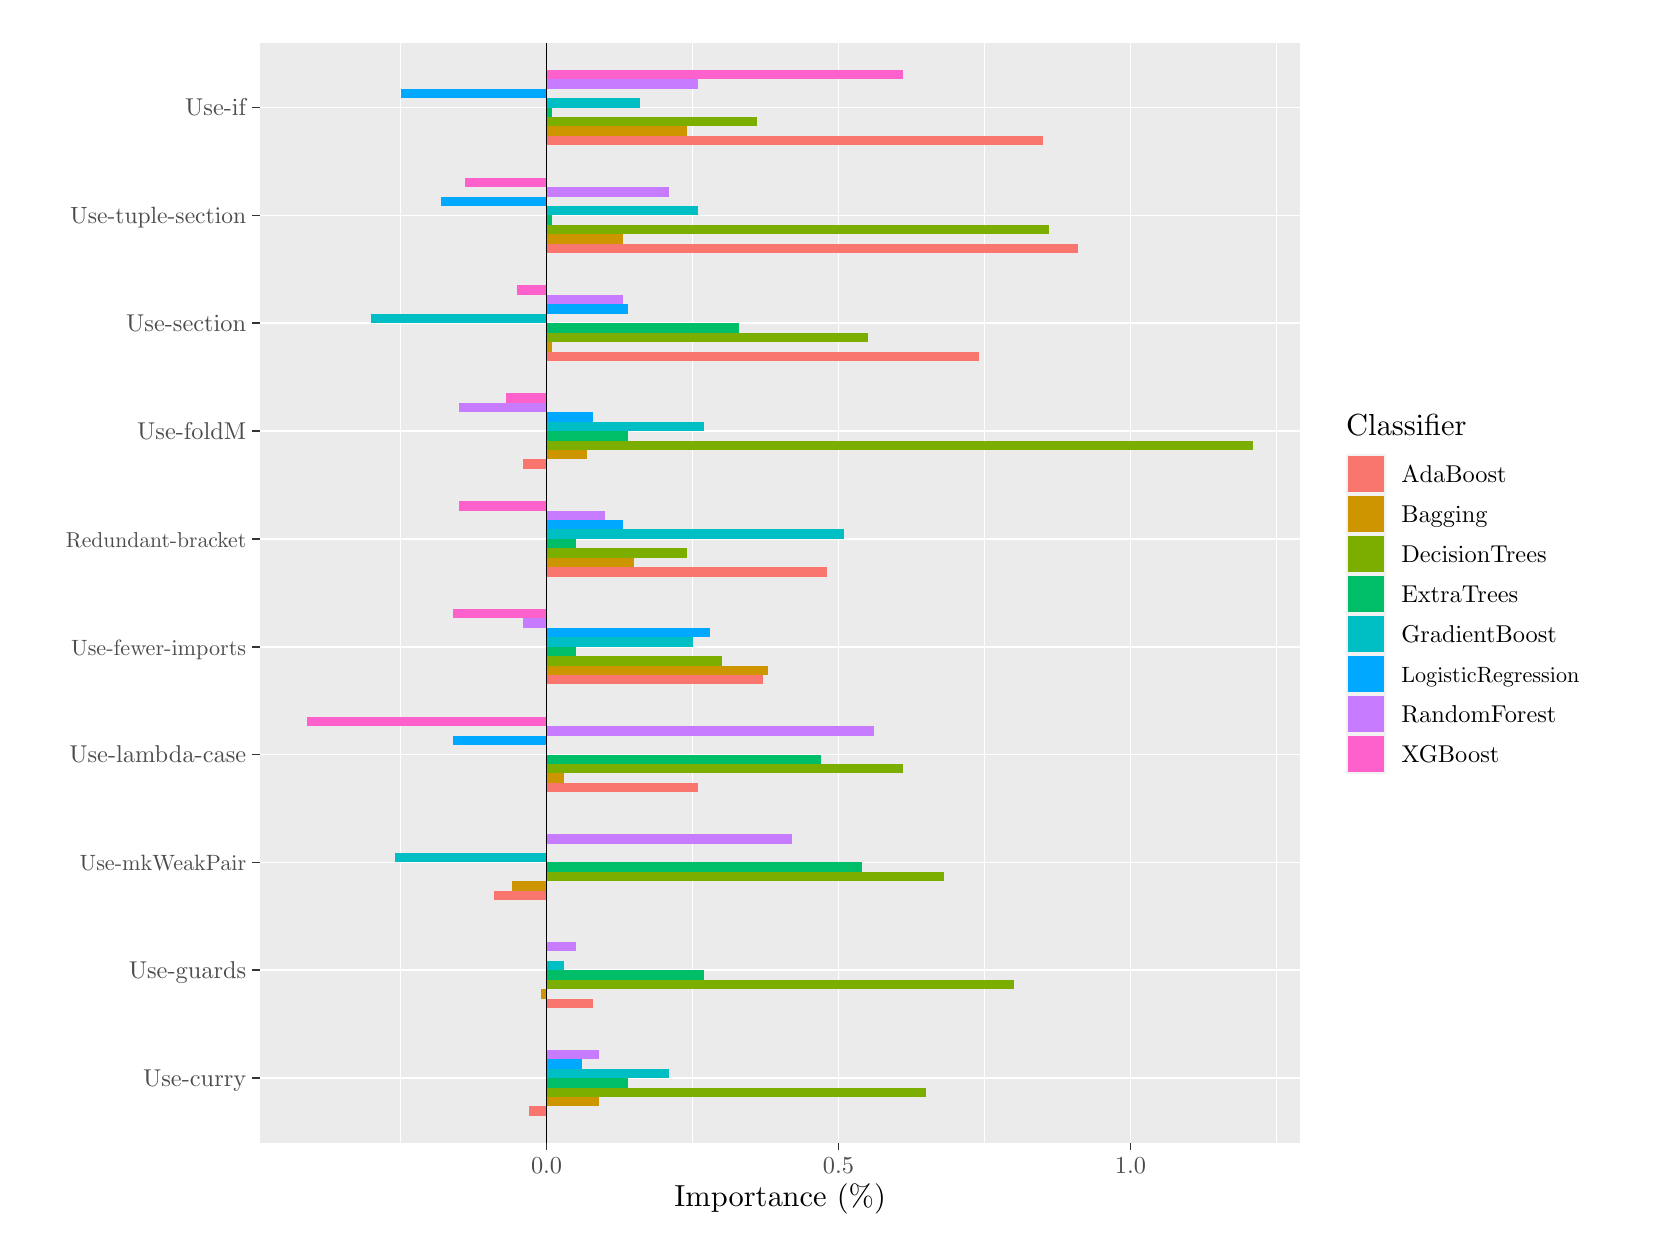
\begin{tikzpicture}[x=1pt,y=1pt]
\definecolor{fillColor}{RGB}{255,255,255}
\path[use as bounding box,fill=fillColor,fill opacity=0.00] (0,0) rectangle (578.16,433.62);
\begin{scope}
\path[clip] (  0.00,  0.00) rectangle (578.16,433.62);
\definecolor{drawColor}{RGB}{255,255,255}
\definecolor{fillColor}{RGB}{255,255,255}

\path[draw=drawColor,line width= 0.6pt,line join=round,line cap=round,fill=fillColor] (  0.00,  0.00) rectangle (578.16,433.62);
\end{scope}
\begin{scope}
\path[clip] ( 83.91, 30.69) rectangle (459.91,428.12);
\definecolor{fillColor}{gray}{0.92}

\path[fill=fillColor] ( 83.91, 30.69) rectangle (459.91,428.12);
\definecolor{drawColor}{RGB}{255,255,255}

\path[draw=drawColor,line width= 0.3pt,line join=round] (134.76, 30.69) --
	(134.76,428.12);

\path[draw=drawColor,line width= 0.3pt,line join=round] (240.26, 30.69) --
	(240.26,428.12);

\path[draw=drawColor,line width= 0.3pt,line join=round] (345.76, 30.69) --
	(345.76,428.12);

\path[draw=drawColor,line width= 0.3pt,line join=round] (451.26, 30.69) --
	(451.26,428.12);

\path[draw=drawColor,line width= 0.6pt,line join=round] ( 83.91, 54.06) --
	(459.91, 54.06);

\path[draw=drawColor,line width= 0.6pt,line join=round] ( 83.91, 93.03) --
	(459.91, 93.03);

\path[draw=drawColor,line width= 0.6pt,line join=round] ( 83.91,131.99) --
	(459.91,131.99);

\path[draw=drawColor,line width= 0.6pt,line join=round] ( 83.91,170.96) --
	(459.91,170.96);

\path[draw=drawColor,line width= 0.6pt,line join=round] ( 83.91,209.92) --
	(459.91,209.92);

\path[draw=drawColor,line width= 0.6pt,line join=round] ( 83.91,248.88) --
	(459.91,248.88);

\path[draw=drawColor,line width= 0.6pt,line join=round] ( 83.91,287.85) --
	(459.91,287.85);

\path[draw=drawColor,line width= 0.6pt,line join=round] ( 83.91,326.81) --
	(459.91,326.81);

\path[draw=drawColor,line width= 0.6pt,line join=round] ( 83.91,365.78) --
	(459.91,365.78);

\path[draw=drawColor,line width= 0.6pt,line join=round] ( 83.91,404.74) --
	(459.91,404.74);

\path[draw=drawColor,line width= 0.6pt,line join=round] (187.51, 30.69) --
	(187.51,428.12);

\path[draw=drawColor,line width= 0.6pt,line join=round] (293.01, 30.69) --
	(293.01,428.12);

\path[draw=drawColor,line width= 0.6pt,line join=round] (398.51, 30.69) --
	(398.51,428.12);
\definecolor{fillColor}{RGB}{248,118,109}

\path[fill=fillColor] (187.51,391.10) rectangle (366.86,394.51);

\path[fill=fillColor] (187.51,352.14) rectangle (379.52,355.55);

\path[fill=fillColor] (187.51,313.18) rectangle (343.65,316.59);

\path[fill=fillColor] (179.07,274.21) rectangle (187.51,277.62);

\path[fill=fillColor] (187.51,235.25) rectangle (288.79,238.66);

\path[fill=fillColor] (187.51,196.28) rectangle (265.58,199.69);

\path[fill=fillColor] (187.51,157.32) rectangle (242.37,160.73);

\path[fill=fillColor] (168.52,118.36) rectangle (187.51,121.76);

\path[fill=fillColor] (187.51, 79.39) rectangle (204.39, 82.80);

\path[fill=fillColor] (181.18, 40.43) rectangle (187.51, 43.84);
\definecolor{fillColor}{RGB}{205,150,0}

\path[fill=fillColor] (187.51,394.51) rectangle (238.15,397.92);

\path[fill=fillColor] (187.51,355.55) rectangle (214.94,358.96);

\path[fill=fillColor] (187.51,316.59) rectangle (189.62,319.99);

\path[fill=fillColor] (187.51,277.62) rectangle (202.28,281.03);

\path[fill=fillColor] (187.51,238.66) rectangle (219.16,242.07);

\path[fill=fillColor] (187.51,199.69) rectangle (267.69,203.10);

\path[fill=fillColor] (187.51,160.73) rectangle (193.84,164.14);

\path[fill=fillColor] (174.85,121.76) rectangle (187.51,125.17);

\path[fill=fillColor] (185.40, 82.80) rectangle (187.51, 86.21);

\path[fill=fillColor] (187.51, 43.84) rectangle (206.50, 47.25);
\definecolor{fillColor}{RGB}{124,174,0}

\path[fill=fillColor] (187.51,397.92) rectangle (263.47,401.33);

\path[fill=fillColor] (187.51,358.96) rectangle (368.97,362.37);

\path[fill=fillColor] (187.51,319.99) rectangle (303.56,323.40);

\path[fill=fillColor] (187.51,281.03) rectangle (442.82,284.44);

\path[fill=fillColor] (187.51,242.07) rectangle (238.15,245.48);

\path[fill=fillColor] (187.51,203.10) rectangle (250.81,206.51);

\path[fill=fillColor] (187.51,164.14) rectangle (316.22,167.55);

\path[fill=fillColor] (187.51,125.17) rectangle (330.99,128.58);

\path[fill=fillColor] (187.51, 86.21) rectangle (356.31, 89.62);

\path[fill=fillColor] (187.51, 47.25) rectangle (324.66, 50.65);
\definecolor{fillColor}{RGB}{0,190,103}

\path[fill=fillColor] (187.51,401.33) rectangle (189.62,404.74);

\path[fill=fillColor] (187.51,362.37) rectangle (189.62,365.78);

\path[fill=fillColor] (187.51,323.40) rectangle (257.14,326.81);

\path[fill=fillColor] (187.51,284.44) rectangle (217.05,287.85);

\path[fill=fillColor] (187.51,245.48) rectangle (198.06,248.88);

\path[fill=fillColor] (187.51,206.51) rectangle (198.06,209.92);

\path[fill=fillColor] (187.51,167.55) rectangle (286.68,170.96);

\path[fill=fillColor] (187.51,128.58) rectangle (301.45,131.99);

\path[fill=fillColor] (187.51, 89.62) rectangle (244.48, 93.03);

\path[fill=fillColor] (187.51, 50.65) rectangle (217.05, 54.06);
\definecolor{fillColor}{RGB}{0,191,196}

\path[fill=fillColor] (187.51,404.74) rectangle (221.27,408.15);

\path[fill=fillColor] (187.51,365.78) rectangle (242.37,369.19);

\path[fill=fillColor] (124.21,326.81) rectangle (187.51,330.22);

\path[fill=fillColor] (187.51,287.85) rectangle (244.48,291.26);

\path[fill=fillColor] (187.51,248.88) rectangle (295.12,252.29);

\path[fill=fillColor] (187.51,209.92) rectangle (240.26,213.33);

\path[fill=fillColor] (187.51,170.96) rectangle (187.51,174.37);

\path[fill=fillColor] (132.65,131.99) rectangle (187.51,135.40);

\path[fill=fillColor] (187.51, 93.03) rectangle (193.84, 96.44);

\path[fill=fillColor] (187.51, 54.06) rectangle (231.82, 57.47);
\definecolor{fillColor}{RGB}{0,169,255}

\path[fill=fillColor] (134.76,408.15) rectangle (187.51,411.56);

\path[fill=fillColor] (149.53,369.19) rectangle (187.51,372.60);

\path[fill=fillColor] (187.51,330.22) rectangle (217.05,333.63);

\path[fill=fillColor] (187.51,291.26) rectangle (204.39,294.67);

\path[fill=fillColor] (187.51,252.29) rectangle (214.94,255.70);

\path[fill=fillColor] (187.51,213.33) rectangle (246.59,216.74);

\path[fill=fillColor] (153.75,174.37) rectangle (187.51,177.78);

\path[fill=fillColor] (187.51,135.40) rectangle (187.51,138.81);

\path[fill=fillColor] (187.51, 96.44) rectangle (187.51, 99.85);

\path[fill=fillColor] (187.51, 57.47) rectangle (200.17, 60.88);
\definecolor{fillColor}{RGB}{199,124,255}

\path[fill=fillColor] (187.51,411.56) rectangle (242.37,414.97);

\path[fill=fillColor] (187.51,372.60) rectangle (231.82,376.01);

\path[fill=fillColor] (187.51,333.63) rectangle (214.94,337.04);

\path[fill=fillColor] (155.86,294.67) rectangle (187.51,298.08);

\path[fill=fillColor] (187.51,255.70) rectangle (208.61,259.11);

\path[fill=fillColor] (179.07,216.74) rectangle (187.51,220.15);

\path[fill=fillColor] (187.51,177.78) rectangle (305.67,181.18);

\path[fill=fillColor] (187.51,138.81) rectangle (276.13,142.22);

\path[fill=fillColor] (187.51, 99.85) rectangle (198.06,103.26);

\path[fill=fillColor] (187.51, 60.88) rectangle (206.50, 64.29);
\definecolor{fillColor}{RGB}{255,97,204}

\path[fill=fillColor] (187.51,414.97) rectangle (316.22,418.38);

\path[fill=fillColor] (157.97,376.01) rectangle (187.51,379.41);

\path[fill=fillColor] (176.96,337.04) rectangle (187.51,340.45);

\path[fill=fillColor] (172.74,298.08) rectangle (187.51,301.49);

\path[fill=fillColor] (155.86,259.11) rectangle (187.51,262.52);

\path[fill=fillColor] (153.75,220.15) rectangle (187.51,223.56);

\path[fill=fillColor] (101.00,181.18) rectangle (187.51,184.59);

\path[fill=fillColor] (187.51,142.22) rectangle (187.51,145.63);

\path[fill=fillColor] (187.51,103.26) rectangle (187.51,106.67);

\path[fill=fillColor] (187.51, 64.29) rectangle (187.51, 67.70);
\definecolor{drawColor}{RGB}{0,0,0}

\path[draw=drawColor,line width= 0.6pt,line join=round] (187.51, 30.69) -- (187.51,428.12);
\end{scope}
\begin{scope}
\path[clip] (  0.00,  0.00) rectangle (578.16,433.62);
\definecolor{drawColor}{gray}{0.30}

\node[text=drawColor,anchor=base east,inner sep=0pt, outer sep=0pt, scale=  0.88] at ( 78.96, 51.03) {Use-curry};

\node[text=drawColor,anchor=base east,inner sep=0pt, outer sep=0pt, scale=  0.88] at ( 78.96, 90.00) {Use-guards};

\node[text=drawColor,anchor=base east,inner sep=0pt, outer sep=0pt, scale=  0.80] at ( 78.96,128.96) {Use-mkWeakPair};

\node[text=drawColor,anchor=base east,inner sep=0pt, outer sep=0pt, scale=  0.88] at ( 78.96,167.93) {Use-lambda-case};

\node[text=drawColor,anchor=base east,inner sep=0pt, outer sep=0pt, scale=  0.80] at ( 78.96,206.89) {Use-fewer-imports};

\node[text=drawColor,anchor=base east,inner sep=0pt, outer sep=0pt, scale=  0.78] at ( 78.96,245.85) {Redundant-bracket};

\node[text=drawColor,anchor=base east,inner sep=0pt, outer sep=0pt, scale=  0.88] at ( 78.96,284.82) {Use-foldM};

\node[text=drawColor,anchor=base east,inner sep=0pt, outer sep=0pt, scale=  0.88] at ( 78.96,323.78) {Use-section};

\node[text=drawColor,anchor=base east,inner sep=0pt, outer sep=0pt, scale=  0.85] at ( 78.96,362.75) {Use-tuple-section};

\node[text=drawColor,anchor=base east,inner sep=0pt, outer sep=0pt, scale=  0.88] at ( 78.96,401.71) {Use-if};
\end{scope}
\begin{scope}
\path[clip] (  0.00,  0.00) rectangle (578.16,433.62);
\definecolor{drawColor}{gray}{0.20}

\path[draw=drawColor,line width= 0.6pt,line join=round] ( 81.16, 54.06) --
	( 83.91, 54.06);

\path[draw=drawColor,line width= 0.6pt,line join=round] ( 81.16, 93.03) --
	( 83.91, 93.03);

\path[draw=drawColor,line width= 0.6pt,line join=round] ( 81.16,131.99) --
	( 83.91,131.99);

\path[draw=drawColor,line width= 0.6pt,line join=round] ( 81.16,170.96) --
	( 83.91,170.96);

\path[draw=drawColor,line width= 0.6pt,line join=round] ( 81.16,209.92) --
	( 83.91,209.92);

\path[draw=drawColor,line width= 0.6pt,line join=round] ( 81.16,248.88) --
	( 83.91,248.88);

\path[draw=drawColor,line width= 0.6pt,line join=round] ( 81.16,287.85) --
	( 83.91,287.85);

\path[draw=drawColor,line width= 0.6pt,line join=round] ( 81.16,326.81) --
	( 83.91,326.81);

\path[draw=drawColor,line width= 0.6pt,line join=round] ( 81.16,365.78) --
	( 83.91,365.78);

\path[draw=drawColor,line width= 0.6pt,line join=round] ( 81.16,404.74) --
	( 83.91,404.74);
\end{scope}
\begin{scope}
\path[clip] (  0.00,  0.00) rectangle (578.16,433.62);
\definecolor{drawColor}{gray}{0.20}

\path[draw=drawColor,line width= 0.6pt,line join=round] (187.51, 27.94) --
	(187.51, 30.69);

\path[draw=drawColor,line width= 0.6pt,line join=round] (293.01, 27.94) --
	(293.01, 30.69);

\path[draw=drawColor,line width= 0.6pt,line join=round] (398.51, 27.94) --
	(398.51, 30.69);
\end{scope}
\begin{scope}
\path[clip] (  0.00,  0.00) rectangle (578.16,433.62);
\definecolor{drawColor}{gray}{0.30}

\node[text=drawColor,anchor=base,inner sep=0pt, outer sep=0pt, scale=  0.88] at (187.51, 19.68) {0.0};

\node[text=drawColor,anchor=base,inner sep=0pt, outer sep=0pt, scale=  0.88] at (293.01, 19.68) {0.5};

\node[text=drawColor,anchor=base,inner sep=0pt, outer sep=0pt, scale=  0.88] at (398.51, 19.68) {1.0};
\end{scope}
\begin{scope}
\path[clip] (  0.00,  0.00) rectangle (578.16,433.62);
\definecolor{drawColor}{RGB}{0,0,0}

\node[text=drawColor,anchor=base,inner sep=0pt, outer sep=0pt, scale=  1.10] at (271.91,  7.64) {Importance (\%)};
\end{scope}
\begin{scope}
\path[clip] (  0.00,  0.00) rectangle (578.16,433.62);
\definecolor{fillColor}{RGB}{255,255,255}

\path[fill=fillColor] (470.91,158.48) rectangle (572.66,300.33);
\end{scope}
\begin{scope}
\path[clip] (  0.00,  0.00) rectangle (578.16,433.62);
\definecolor{drawColor}{RGB}{0,0,0}

\node[text=drawColor,anchor=base west,inner sep=0pt, outer sep=0pt, scale=  1.10] at (476.41,286.18) {Classifier};
\end{scope}
\begin{scope}
\path[clip] (  0.00,  0.00) rectangle (578.16,433.62);
\definecolor{fillColor}{gray}{0.95}

\path[fill=fillColor] (476.41,265.16) rectangle (490.86,279.61);
\end{scope}
\begin{scope}
\path[clip] (  0.00,  0.00) rectangle (578.16,433.62);
\definecolor{fillColor}{RGB}{248,118,109}

\path[fill=fillColor] (477.12,265.87) rectangle (490.15,278.90);
\end{scope}
\begin{scope}
\path[clip] (  0.00,  0.00) rectangle (578.16,433.62);
\definecolor{fillColor}{gray}{0.95}

\path[fill=fillColor] (476.41,250.70) rectangle (490.86,265.16);
\end{scope}
\begin{scope}
\path[clip] (  0.00,  0.00) rectangle (578.16,433.62);
\definecolor{fillColor}{RGB}{205,150,0}

\path[fill=fillColor] (477.12,251.42) rectangle (490.15,264.45);
\end{scope}
\begin{scope}
\path[clip] (  0.00,  0.00) rectangle (578.16,433.62);
\definecolor{fillColor}{gray}{0.95}

\path[fill=fillColor] (476.41,236.25) rectangle (490.86,250.70);
\end{scope}
\begin{scope}
\path[clip] (  0.00,  0.00) rectangle (578.16,433.62);
\definecolor{fillColor}{RGB}{124,174,0}

\path[fill=fillColor] (477.12,236.96) rectangle (490.15,249.99);
\end{scope}
\begin{scope}
\path[clip] (  0.00,  0.00) rectangle (578.16,433.62);
\definecolor{fillColor}{gray}{0.95}

\path[fill=fillColor] (476.41,221.80) rectangle (490.86,236.25);
\end{scope}
\begin{scope}
\path[clip] (  0.00,  0.00) rectangle (578.16,433.62);
\definecolor{fillColor}{RGB}{0,190,103}

\path[fill=fillColor] (477.12,222.51) rectangle (490.15,235.54);
\end{scope}
\begin{scope}
\path[clip] (  0.00,  0.00) rectangle (578.16,433.62);
\definecolor{fillColor}{gray}{0.95}

\path[fill=fillColor] (476.41,207.34) rectangle (490.86,221.80);
\end{scope}
\begin{scope}
\path[clip] (  0.00,  0.00) rectangle (578.16,433.62);
\definecolor{fillColor}{RGB}{0,191,196}

\path[fill=fillColor] (477.12,208.05) rectangle (490.15,221.08);
\end{scope}
\begin{scope}
\path[clip] (  0.00,  0.00) rectangle (578.16,433.62);
\definecolor{fillColor}{gray}{0.95}

\path[fill=fillColor] (476.41,192.89) rectangle (490.86,207.34);
\end{scope}
\begin{scope}
\path[clip] (  0.00,  0.00) rectangle (578.16,433.62);
\definecolor{fillColor}{RGB}{0,169,255}

\path[fill=fillColor] (477.12,193.60) rectangle (490.15,206.63);
\end{scope}
\begin{scope}
\path[clip] (  0.00,  0.00) rectangle (578.16,433.62);
\definecolor{fillColor}{gray}{0.95}

\path[fill=fillColor] (476.41,178.43) rectangle (490.86,192.89);
\end{scope}
\begin{scope}
\path[clip] (  0.00,  0.00) rectangle (578.16,433.62);
\definecolor{fillColor}{RGB}{199,124,255}

\path[fill=fillColor] (477.12,179.15) rectangle (490.15,192.18);
\end{scope}
\begin{scope}
\path[clip] (  0.00,  0.00) rectangle (578.16,433.62);
\definecolor{fillColor}{gray}{0.95}

\path[fill=fillColor] (476.41,163.98) rectangle (490.86,178.43);
\end{scope}
\begin{scope}
\path[clip] (  0.00,  0.00) rectangle (578.16,433.62);
\definecolor{fillColor}{RGB}{255,97,204}

\path[fill=fillColor] (477.12,164.69) rectangle (490.15,177.72);
\end{scope}
\begin{scope}
\path[clip] (  0.00,  0.00) rectangle (578.16,433.62);
\definecolor{drawColor}{RGB}{0,0,0}

\node[text=drawColor,anchor=base west,inner sep=0pt, outer sep=0pt, scale=  0.88] at (496.36,269.35) {AdaBoost};
\end{scope}
\begin{scope}
\path[clip] (  0.00,  0.00) rectangle (578.16,433.62);
\definecolor{drawColor}{RGB}{0,0,0}

\node[text=drawColor,anchor=base west,inner sep=0pt, outer sep=0pt, scale=  0.88] at (496.36,254.90) {Bagging};
\end{scope}
\begin{scope}
\path[clip] (  0.00,  0.00) rectangle (578.16,433.62);
\definecolor{drawColor}{RGB}{0,0,0}

\node[text=drawColor,anchor=base west,inner sep=0pt, outer sep=0pt, scale=  0.88] at (496.36,240.45) {DecisionTrees};
\end{scope}
\begin{scope}
\path[clip] (  0.00,  0.00) rectangle (578.16,433.62);
\definecolor{drawColor}{RGB}{0,0,0}

\node[text=drawColor,anchor=base west,inner sep=0pt, outer sep=0pt, scale=  0.88] at (496.36,225.99) {ExtraTrees};
\end{scope}
\begin{scope}
\path[clip] (  0.00,  0.00) rectangle (578.16,433.62);
\definecolor{drawColor}{RGB}{0,0,0}

\node[text=drawColor,anchor=base west,inner sep=0pt, outer sep=0pt, scale=  0.88] at (496.36,211.54) {GradientBoost};
\end{scope}
\begin{scope}
\path[clip] (  0.00,  0.00) rectangle (578.16,433.62);
\definecolor{drawColor}{RGB}{0,0,0}

\node[text=drawColor,anchor=base west,inner sep=0pt, outer sep=0pt, scale=  0.80] at (496.36,197.08) {LogisticRegression};
\end{scope}
\begin{scope}
\path[clip] (  0.00,  0.00) rectangle (578.16,433.62);
\definecolor{drawColor}{RGB}{0,0,0}

\node[text=drawColor,anchor=base west,inner sep=0pt, outer sep=0pt, scale=  0.88] at (496.36,182.63) {RandomForest};
\end{scope}
\begin{scope}
\path[clip] (  0.00,  0.00) rectangle (578.16,433.62);
\definecolor{drawColor}{RGB}{0,0,0}

\node[text=drawColor,anchor=base west,inner sep=0pt, outer sep=0pt, scale=  0.88] at (496.36,168.18) {XGBoost};
\end{scope}
\end{tikzpicture}
